

\subsection{Iteración 2}

En esta sección se van a llevar a cabo pruebas con usuarios reales para analizar la eficacia y usabilidad del sistema desarrollado. Para esto se ha creado un cuestionario del que se hablará a continuación y se ha presentado a los usuarios con el juego para que realicen 5 pruebas cada uno. Los usuarios varían tanto en edad y sexo, como en conocimientos tecnológicos previos para obtener información más amplia.



\subsubsection{Cuestionario}

Para evaluar la usabilidad del sistema se ha optado por utilizar un cuestionario SUS (System Usability Scale) ya que se trata de un sistema estándar el el desarrollo de software para medir la calidad y usabilidad de un programa. Se entiende como usabilidad la capacidad del programa para ser comprendido y utilizado por una persona.

Esta es una métrica fundamental en este proyecto, ya que un sistema poco usable, aunque tuviera una gran efectividad, reduciría drásticamente su calidad al dificultar su uso y entendimiento para el usuario. Por desgracia, para este proyecto no se dispone de los conocimientos, profesionales, tiempo ni usuarios para poder hacer un buen análisis de su efectividad y eficacia como sistema contra el deterioro cognitivo leve o para el entrenamiento cognitivo en general.

Por estos motivo, para el ámbito de este proyecto, solo se va a estudiar la usabilidad y todas las opiniones o pensamientos que ofrezcan los participantes.

El cuestionario que se les ha presentado a los usuarios se encuentra detallado en el apéndice \textbf{Cuestionarios} (\ref{sec:apendice:Custionarios}). Se trata de un cuestionario estándar con 10 preguntas a las que se responde con un número entre el 1 y el 5 indicando el grado con el que los usuarios están o no de acuerdo con el enunciado, significando un 1 que están totalmente en desacuerdo, y un 5 que están totalmente de acuerdo. Este método de evaluación se conoce como la escala Linkert y permite obtener un resultado más preciso de las opiniones del usuario al ofrecerle poder expresar su grado exacto de concordancia con los enunciados, además de permitir cuantificar numéricamente las respuestas de cada usuario para posterior análisis \cite{DES_5_2_linkert}.


El cuestionario, siguiendo el estándar SUS contiene diez enunciados, cinco de los cuales son positivos y el resto negativos. Dichos enunciados se presentan de forma alterna para hacer el test lo más homogéneo posible y limitar el sesgo. Una vez respondidos los cuestionarios, se puede obtener una calificación entre 0 y 100 puntos mediante una fórmula matemática sencilla:

\begin{itemize}
	\item{Sumar los resultados de los enunciados positivos y restar 5.}
	
	\item{Restar a 25 la suma de los enunciados negativos.}
	
	\item{Por último, sumar los dos números anteriores y multiplicar el resultado por 2,5.}
	
\end{itemize}

De esta forma, se obtiene un resultado que puede puntuar la usabilidad del sistema según el usuario. Aunque la escala es lineal entre 0 y 100, solo se considera que un sistema tiene una buena usabilidad si su puntuación en el test SUS supera los 68 puntos.

\subsubsection{Pruebas}

Las pruebas que se han realizado consisten en una sesión de juego de una duración de 5 minutos aproximandamente. Las personas seleccionadas para llevar a cabo estas pruebas pertenecen a distintos grupos de edad, conocimientos tecnológicos y familiaridad con la realidad virtual.

Un total de seis personas han prestado su ayuda para este estudio, las cuales se pueden clasificar de la siguiente forma:

\begin{itemize}
	\item{\textbf{Edad}. Tres personas tienen entre 20 y 30 años. Otras 3 tienen más de 60 años.}
	
	\item{\textbf{Conocimientos tecnológicos}. Cuatro personas tienen al menos conocimientos tecnológicos básicos, dos de las cuales tienen conocimientos avanzados. Otras dos personas no tienen conocimientos tecnológicos.}
	
	\item{\textbf{Familiaridad RV}. Dos personas están familiarizadas con la realidad virtual por experiencias previas. Para otras cuatro personas, esta ha sido su primera experiencia en realidad virtual.}
	
\end{itemize}

A cada persona se le ha asignado una letra (de la A a la F) para diferenciarlos y proteger su identidad. Para ver como se distribuyen en concreto estas personas en los tres grupos anteriores, se ha creado la tabla de la figura \ref{fig:tablaPersonasLetras} en la que se pueden ver cada una de las personas encuestadas clasificadas en las tres categorías, según edad, conocimiento tecnológico y si están familiarizadas con la RV o no.


%\begin{figure}
%	\centering
%	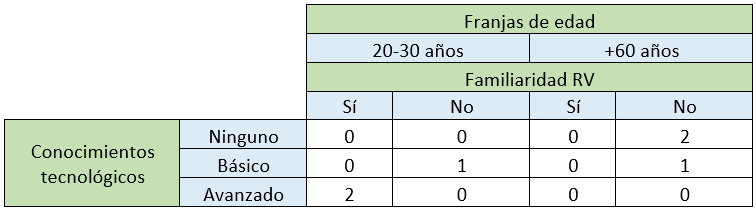
\includegraphics[width=0.7\textwidth]{04.Desarrollo/05.Entrega5/02.Iteracion5_2/00.Figuras/01.tabla_personas.png}
%	\caption{Número de personas encuestadas divididas por grupos de edad, conocimientos tecnológicos y familiaridad con la RV.}
%	\label{fig:tablaPersonas}
%\end{figure}


\begin{figure}
	\centering
	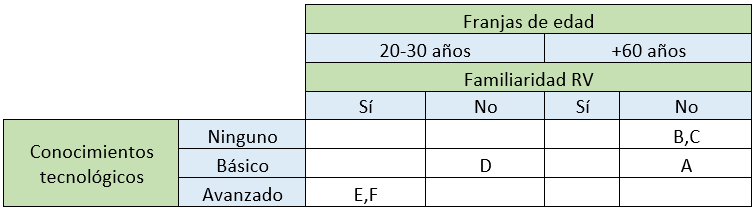
\includegraphics[width=0.7\textwidth]{04.Desarrollo/05.Entrega5/02.Iteracion5_2/00.Figuras/02.tabla_personas_letras.png}
	\caption{Personas encuestadas identificadas por letras y divididas por grupos de edad, conocimientos tecnológicos y familiaridad con la RV.}
	\label{fig:tablaPersonasLetras}
\end{figure}


A todas las personas se les ha dado una explicación de la motivación y objetivo del juego, así como de los controles y todo lo que necesitan saber para poder utilizar el juego. En todo momento durante las pruebas las personas han estado acompañadas y, en caso de ser necesario, aconsejadas sobre como actuar o avanzar en el juego.

Aunque el juego y las gafas de RV permiten el uso de forma completamente independiente, las pruebas se han realizado con un cable uniendo las gafas a un ordenador desde el que poder monitorizar lo que ve y hace el jugador, así como poder realizar grabaciones de vídeo para posterior estudio.


En el repositorio de Github en el que se encuentra este proyecto (\url{https://github.com/Eltrio723/TFG}), están disponibles algunos vídeos de las pruebas realizadas.


\subsubsection{Resultados}
\label{sec:e5i2:res}

Tras realizar las pruebas, contabilizar los cuestionarios y analizar toda la información proporcionada por los usuarios se llega a varias conclusiones y datos notables que se van a detallar a continuación.

En primer lugar se muestra una tabla (tabla \ref{tab:resultados_usabilidad__entrega}) con los resultados obtenidos en los cuestionarios realizados, donde aparecen por cada fila todas las respuestas de cada usuario y en las tres últimas columnas aparecen los cálculos habituales de los cuestionarios SUS, incluyendo en la columna final, la puntuación total de usabilidad que ese usuario otorga al sistema.



\begin{table}[H]
	\centering
	\resizebox{\textwidth}{!}{%
		\begin{tabular}{|l|l|l|l|l|l|l|l|l|l|l|l|l|l|}
			\hline
			Encuestado & Preg. 1 & Preg. 2 & Preg. 3 & Preg. 4 & Preg. 5 & Preg. 6 & Preg. 7 & Preg. 8 & Preg. 9 & Preg. 10 & Suma impares & Suma pares & Total SUS \\ \hline
			A & 4 & 3 & 4 & 4 & 4 & 2 & 4 & 2 & 2 & 3 & 18 & 14 & 60 \\ \hline
			B & 5 & 1 & 5 & 4 & 5 & 2 & 5 & 1 & 5 & 2 & 25 & 10 & 87.5 \\ \hline
			C & 4 & 1 & 4 & 3 & 4 & 2 & 4 & 2 & 3 & 2 & 19 & 10 & 72.5 \\ \hline
			D & 4 & 1 & 5 & 2 & 4 & 2 & 4 & 2 & 4 & 1 & 21 & 8 & 82.5 \\ \hline
			E & 4 & 2 & 4 & 1 & 4 & 2 & 5 & 2 & 4 & 1 & 21 & 8 & 82.5 \\ \hline
			F & 4 & 1 & 5 & 3 & 5 & 1 & 4 & 1 & 5 & 1 & 23 & 7 & 90 \\ \hline
		\end{tabular}%
	}
	\caption{Resultados de usabilidad obtenidos tras las pruebas}
	\label{tab:resultados_usabilidad__entrega}
\end{table}



Estudiando esta tabla de resultados se puede ver que la mayoría de las preguntas reciben una puntuación similar entre los usuarios. Las preguntas con más variación son la 4 y la 9.

El enunciado 4 es el siguiente: "Creo que necesitaría el apoyo de otra persona para poder utilizar este juego.". Las personas que están en desacuerdo con esta pregunta son las D y E, ambas en la franja de edad más joven, mientras que las personas más de acuerdo son la A y B, ambas de la franja de edad superior. 

Para la pregunta 9: "Me sentí muy seguro usando el sistema.", las respuestas son dispares pero no necesariamente se pueden clasificar dentro de uno de los grupos. Por ejemplo, de las tres personas de mayor edad, dos están en desacuerdo o neutro, pero la otra está totalmente de acuerdo con el enunciado.

La familiaridad con la realidad virtual tampoco parece ser un factor decisivo, sin embargo, la edad vuelve a crear una distinción en la pregunta 10, dónde las personas más jóvenes piensan que no necesitan aprender nada antes de comenzar a jugar, en lugar de las personas mayores, que están menos de acuerdo, aunque no por una gran diferencia.

En el grupo de personas para este estudio, el grado de conocimientos tecnológicos tiene correlación con la edad, esto es algo bastante habitual hoy en día, pero puede estar enmascarando algunos resultados atribuidos inicialmente al factor de edad.

Todas las personas tras la prueba afirman que la realidad virtual les ha gustado y en ningún caso se han sentido mareados o desorientados. Tras probar experiencias de RV externas a este proyecto y con más movimiento, dos de las personas se sintieron mareadas, aunque no sucedió lo mismo con el resto, que siguieron cómodas en la RV. 

De esto se puede deducir que este juego difícilmente producirá mareos puesto que tiene un ritmo lento y es estático, sin movimientos bruscos. Esto es una gran ventaja para el objetivo que se desea para este proyecto. Por este mismo motivo, es posible que la familiarización con la realidad virtual previa de cada persona no afecte a los resultados obtenidos.

Finalmente, teniendo en cuenta las puntuaciones de los cuestionarios, solo una persona indica una usabilidad  por debajo del valor aceptable de 68 (figura \ref{fig:MU_sus_entrega}), en este caso: 60. Aunque está puntuación sigue estando dentro de la franja marginal. 

Uniendo todos los resultados para calcular una media, se obtiene que la puntuación de usabilidad para este proyecto en esta prueba es de 79 puntos. Esta puntuación está dentro del rango aceptable y nos indica que el sistema creado es percibido por los usuarios como fácil de utilizar y seguro. Por tanto, se puede decir que la realidad virtual es una buena tecnología para utilizar con distintos tipos de personas y que el juego desarrollado en concreto es fácil de entender, coherente y ha gustado a los usuarios.

\begin{figure}
	\centering
	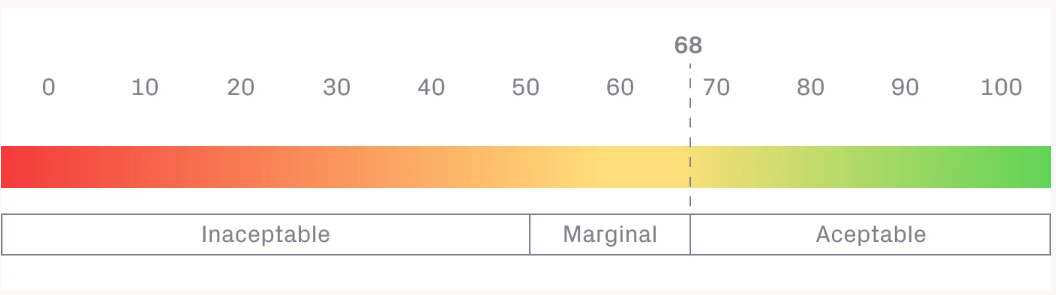
\includegraphics[width=0.5\textwidth]{03.EstudioProblema/04.MetodologiaAUsar/00.Figuras/03.sus.png}
	\caption{Representación de los resultados de un SUS. \cite{MU_eval_sus}}
	\label{fig:MU_sus_entrega}
\end{figure}


Es necesario recordar en este punto, que no se está pretendiendo medir la eficacia del propio entrenamiento cognitivo, en primer lugar porque es una cuestión en la que aún los estudios no se ponen de acuerdo (como se comenta en la sección \ref{sec:estadoArteEficaciaEntrenamientos}), y en segundo lugar, porque está fuera de mis capacidades, conocimientos y del alcance esperado y definido para este proyecto.



\subsubsection{Opinión profesional}


Una de las personas encuestadas se trata de la psicóloga Carmen Granero Rico, especializada en gerontología y con años de experiencia como directora de residencias de mayores. A parte de su participación en la prueba, también ha ofrecido su opinión como profesional del sector y de la cual se presentan fragmentos a continuación:


``La estimulación cognitiva que tú estás haciendo de cara a una persona ya con inicio de deterioro, que ya lo tenemos a partir de una determinada edad, para eso, tu prueba es muy básica. Ahora mismo muy básica porque es lo que tú puedes hacer para tu proyecto, pero si tú ahí te pones con un profesional que sabe de lo que tiene que meter de contenido, puede estar muy bien. Lo que es la parte técnica está, ahora ya hay que meterle los contenidos necesarios para estimular las diferentes áreas y las diferentes habilidades que se necesitan estimular.''

``Podría haber pruebas globales que entrenen todos los aspectos y luego pruebas más especificas.''

``Me ha gustado mucho usar las manos para manejar todo, especialmente el gesto con el pulgar y el índice para seleccionar, porque ese es un movimiento de motricidad fina, y las personas mayores es algo que suelen perder, sobretodo cuando comienzan a tener artritis y artrosis.''

``(la realidad virtual) ... sí que es verdad que es un shock para las personas mayores. También depende de la generación. Por ejemplo, para mi generación es perfectamente soportable y lo puede hacer, pero entiendo que por ejemplo, la generación anterior a la mía no puede. Entre otras cosas porque cuando te pones las gafas pierdes el equilibrio, y ellos de por sí no suelen tener mucho equilibrio.''

``Es una buena base, luego ya es meterle contenido hecho con profesionales de la cognitividad.''

``Esto sirve no solo para personas mayores, también para gente de todas las edades, como los juegos de brain training que teníamos...''

``El estrés, o cualquier tema emocional como la depresión, afectan muchísimo a la memoria, la concentración y la percepción, entonces esto (el juego) puede ser un estímulo en cualquier momento.''











